\documentclass[11pt,a4paper]{article}
\usepackage[utf8]{inputenc}
\usepackage[T1]{fontenc}
\usepackage[french]{babel}
\usepackage{lmodern}
\usepackage{geometry}
\geometry{margin=2.3cm}
\usepackage{microtype}
\usepackage{setspace}
\setstretch{1.1}
\usepackage{xcolor}
\definecolor{cpblue}{HTML}{244A73}
\definecolor{cpgreen}{HTML}{2E7D6E}
\definecolor{cporange}{HTML}{C06B28}
\definecolor{cpgray}{HTML}{F3F5F7}
\definecolor{cpdark}{HTML}{24313B}
\usepackage{tikz}
\usetikzlibrary{arrows.meta,positioning}
\usepackage{booktabs}
\usepackage{tabularx}
\usepackage{array}
\usepackage{amsmath,amssymb}
\usepackage{enumitem}
\setlist{itemsep=1pt,topsep=3pt,parsep=0pt}
\usepackage{hyperref}
\hypersetup{colorlinks=true,linkcolor=cpblue,urlcolor=cpblue,citecolor=cpblue}
\usepackage{fancyhdr}
\usepackage{graphicx}
\usepackage{float}
\usepackage{caption}
\captionsetup{font=small,labelfont=bf}
\pagestyle{fancy}
\fancyhf{}
\lhead{\small Réponses à l'encadrement}
\rhead{\small Prophet, $\alpha_j$, optimisation}
\cfoot{\small\thepage}
\setlength{\headheight}{14pt}
\usepackage{titlesec}
\titleformat{\section}{\large\bfseries\color{cpblue}}{\thesection}{0.5em}{}
\titleformat{\subsection}{\normalsize\bfseries\color{cpdark}}{\thesubsection}{0.5em}{}
\titlespacing*{\section}{0pt}{14pt}{7pt}
\titlespacing*{\subsection}{0pt}{10pt}{5pt}
\newcommand{\code}[1]{\texttt{#1}}

\begin{document}

\begin{center}
{\Large\bfseries\color{cpblue} Prévision Prophet, facteur de confiance et démarche d'optimisation\par}
\vspace{0.2cm}
{\normalsize Module DataCo du modèle SCONTO-SVU\par}
\end{center}
\vspace{0.3cm}

\noindent Ce document répond à trois questions : comment Prophet est-il construit, utilisé et intégré à DataCo ; comment justifier le facteur de recalibration $\alpha_j=\sqrt{j/N}$ ; comment la démarche d'optimisation de SCONTO-SVU est-elle conduite et validée. Les résultats numériques cités proviennent du run de référence RUN 1 (\code{simToRealSeconds = 3600}).

\section{Prévision de la demande avec Prophet}

\subsection{Dataset DataCo et année cible}

Le pipeline DataCo utilise le dataset DataCo Supply Chain, un jeu de données réel de 180\,519 lignes réparties sur 53 colonnes, couvrant les commandes clients, les produits, les délais de livraison, les statuts et les informations géographiques sur la période 2015--2018. Chaque ligne représente une ligne de commande (\emph{order item}). Les champs exploités sont \code{Order Id}, \code{Product Name}, \code{Order Item Quantity}, \code{Order Status}, \code{Order Date}, \code{Days for Shipping Real}, \code{Days for Shipment Scheduled} et \code{Product Price} ; ce dernier fournit un contexte économique mais n'entre pas dans le calcul de la demande.

\begin{center}
\small
\begin{tabular}{lrrl}
\toprule
Année & Lignes & Produits & Rôle \\
\midrule
2015 & 62\,650 & 54 & Apprentissage Prophet \\
2016 & 62\,550 & 54 & Apprentissage Prophet \\
2017 & 53\,196 & 118 & Année cible, catalogue élargi \\
2018 & 2\,123 & 10 & Couverture insuffisante, écartée \\
\bottomrule
\end{tabular}
\end{center}

2015 et 2016 servent à l'apprentissage de Prophet. 2017 contient des observations sur les douze mois, un volume représentatif d'environ 53\,000 lignes valides et un catalogue élargi à 118 produits, le double des deux années précédentes : c'est l'année cible retenue pour la prévision et pour l'exécution de la campagne. Le dernier trimestre de cette année cible présente une forte contraction du volume de commandes par rapport aux neuf premiers mois ; cette contraction est une caractéristique de la campagne 2017, pas une saisonnalité structurelle reproductible d'une année sur l'autre, et constitue le cas le plus exigeant pour l'algorithme de recalibration. 2018 ne couvre que 2\,123 lignes et 10 produits sur l'année et n'est pas retenue.

\subsection{Préparation des données}

Le dataset comporte neuf statuts de commande. Le filtrage vise à conserver les commandes pouvant générer un flux logistique réel.

\begin{center}
\small
\begin{tabular}{ll}
\toprule
Retenus (six statuts) & Exclus (trois statuts) \\
\midrule
\code{COMPLETE}, \code{PENDING\_PAYMENT}, & \code{SUSPECTED\_FRAUD}, \code{CANCELED}, \\
\code{PROCESSING}, \code{PENDING}, & \code{PAYMENT\_REVIEW} \\
\code{CLOSED}, \code{ON\_HOLD} & \\
\bottomrule
\end{tabular}
\end{center}

Les lignes retenues représentent 170\,872 lignes sur 180\,519, soit 94,66\,\%. Les enregistrements retenus sont ensuite regroupés par jour calendaire pour former la série temporelle utilisée par Prophet.

Trois granularités de produit coexistent dans la chaîne et ne doivent pas être confondues. Le dataset DataCo 2017 recense 118 références observées (champ \code{Product Name}). Certains artefacts Prophet historiques sont calculés à une granularité intermédiaire allant jusqu'à neuf produits. Le scénario AnyLogic courant simplifie cette granularité à trois familles expérimentales, \code{DATACO\_SPORTS}, \code{DATACO\_CLOTHING} et \code{DATACO\_ELECTRONICS}. L'affectation d'une commande à une famille est cyclique dans le scénario courant, fondée sur le numéro de commande, et n'est pas un mapping direct du champ \code{Product Name} : les 118 références source ne sont donc pas réparties individuellement sur les trois familles simulées.

\subsection{Entraînement Prophet}

Prophet décompose une série temporelle en composantes additives \cite{taylor2018forecasting} :
\[
y(t) = g(t) + s(t) + h(t) + \varepsilon_t
\]
où $g(t)$ porte la tendance, $s(t)$ la saisonnalité, $h(t)$ l'effet d'éventuels événements calendaires et $\varepsilon_t$ le résidu. Prophet est entraîné sur 2015--2016 puis produit sa prévision pour 2017. Entraîner Prophet sur les deux années qui précèdent l'année cible, plutôt que d'utiliser la demande réelle 2017 elle-même comme prévision initiale, place le Recalibrator devant un écart réel à corriger et permet d'observer l'apport de la recalibration.

\begin{center}
\small
\begin{tabular}{ll}
\toprule
Paramètre & Valeur \\
\midrule
\code{weekly\_seasonality} & \code{True} \\
\code{yearly\_seasonality} & \code{True} \\
\code{changepoint\_prior\_scale} & 0,05 (valeur par défaut) \\
\code{seasonality\_mode} & non fourni explicitement $\to$ mode additif par défaut \\
Calendrier \code{holidays} & non activé \\
\bottomrule
\end{tabular}
\end{center}

Le \code{changepoint\_prior\_scale} gouverne la flexibilité de la tendance aux points de rupture : une valeur plus faible produit une tendance plus lisse, une valeur plus élevée laisse la tendance s'adapter plus fortement aux variations récentes. Le protocole expérimental de campagne retient 2015--2016 pour l'apprentissage et 2017 comme année cible ; la fenêtre de backtest présente dans le notebook de validation constitue une procédure distincte d'évaluation, indépendante de la campagne exécutée dans AnyLogic.

\subsection{Intégration dans AnyLogic}

Le pipeline de préparation produit cinq fichiers, dont seuls les deux derniers sont consommés au runtime par la version DataCo actuellement chargée dans AnyLogic.

\begin{center}
\small
\begin{tabularx}{\textwidth}{>{\ttfamily}p{5.6cm} X}
\toprule
Fichier & Statut \\
\midrule
Prevision\_Annuelle\_\allowbreak Globale\_Daily\_2017.xlsx & Consommé au runtime : prévision globale, chargée dans \code{prophetDailyForecast} puis agrégée par mois \\
dataco\_calibration\_\allowbreak quotidienne\_2017.xlsx & Consommé au runtime : calibration de l'AutoCommande \\
Prevision\_Annuelle\_\allowbreak Par\_Produits\_2017.xlsx & Produit par le pipeline, non chargé \\
Prevision\_30J\_\allowbreak Court\_Terme\_2017.xlsx & Produit par le pipeline, non chargé \\
Prevision\_Mensuelle\_\allowbreak Prophet\_2017.xlsx & Produit par le pipeline, non chargé \\
\bottomrule
\end{tabularx}
\end{center}

Trois structures se répartissent ensuite les rôles de la prévision au fil de la campagne : \code{prophetForecastsOriginal} porte la baseline mensuelle, immuable ; \code{prophetForecasts} est la copie de travail utilisée comme ancre par le Recalibrator ; \code{forecastRecalibreMensuel} porte la prévision recalibrée. Cette dernière n'est jamais réécrite dans les deux premières, ce qui empêche l'accumulation récursive des corrections d'un cycle à l'autre.

\begin{figure}[H]
\centering
\begin{tikzpicture}[>=Latex,node distance=7mm]
\tikzset{
 n/.style={draw=cpdark,rounded corners,fill=cpgray,minimum width=13.5cm,minimum height=8mm,align=center,font=\small},
 a/.style={->,thick}
}
\node[n] (p1) {DataCo brut (180\,519 lignes) $\to$ filtrage des statuts $\to$ agrégation journalière};
\node[n,below=of p1] (p2) {Apprentissage Prophet sur 2015--2016 $\to$ prévision journalière 2017};
\node[n,below=of p2] (p3) {Export Excel $\to$ chargement AnyLogic (\code{prophetDailyForecast}) $\to$ agrégation mensuelle};
\node[n,below=of p3] (p4) {AutoCommande DataCo $\to$ \code{CommandeAgent} $\to$ pipeline Source/Make/Deliver $\to$ demande réelle};
\node[n,below=of p4] (p5) {Recalibrator : combinaison de Prophet et de la demande observée};
\foreach \i/\j in {p1/p2,p2/p3,p3/p4,p4/p5}{\draw[a] (\i)--(\j);}
\end{tikzpicture}
\caption{Chaîne DataCo $\to$ Prophet $\to$ AnyLogic $\to$ Recalibrator.}
\label{fig:pipeline}
\end{figure}

\subsection{AutoCommande et demande réelle simulée}

Le mode DataCo génère une commande cliente agrégée par journée simulée. Le fichier de calibration journalière fournit une quantité moyenne journalière $\mu_m$ pour chaque mois ; la quantité effectivement injectée est tirée selon une loi normale centrée sur cette moyenne :
\[
Q_j \sim \mathcal{N}\!\left(\mu_m,\,(0{,}10\,\mu_m)^2\right)
\]
bornée à une valeur strictement positive. Le système garantit une génération au plus par date simulée. La quantité $Q_j$ est injectée par \code{genererCommandeDataCoPourDate()}, qui appelle la fonction de génération de commande existante \code{genererCommande()} : aucune commande n'est créée en dehors du pipeline normal. La commande devient une \code{CommandeAgent} qui traverse le pipeline Source, Make, Deliver déjà validé, puis alimente la demande réelle mensuelle consommée par le Recalibrator.

\subsection{Résultats du RUN 1}

Les résultats numériques présentés ici proviennent exclusivement du run de référence (RUN 1, \code{simToRealSeconds = 3600}). Au terme de la campagne de génération de la demande, 365 commandes clientes ont été générées, pour une demande totale de 99\,896 unités. Au snapshot relevé, 79 commandes sont closes, dont 20 closes en retard, et 286 restent EN\_ATTENTE ; 22\,469 unités ont été livrées. Le Performance Index au snapshot est de 8,871/10 : cette valeur est un \textbf{snapshot intermédiaire}, non un résultat terminal (section~\ref{sec:condition-terminale}).

\begin{center}
\small
\begin{tabular}{lrr}
\toprule
Indicateur & Prophet & Recalibrator \\
\midrule
Erreur absolue totale & 29\,902,69 & 1\,476,68 \\
MAE mensuelle & 2\,491,89 & 123,06 \\
MAPE & 45,75\,\% & 1,91\,\% \\
RMSE & 3\,441,15 & 180,71 \\
Biais moyen signé & +2\,491,89 & +110,74 \\
\bottomrule
\end{tabular}
\end{center}

La réduction de l'erreur absolue totale atteint environ 95,06\,\%, soit environ 20,25 fois moins d'erreur absolue cumulée pour le Recalibrator que pour Prophet sur cette campagne.

\begin{figure}[H]
\centering
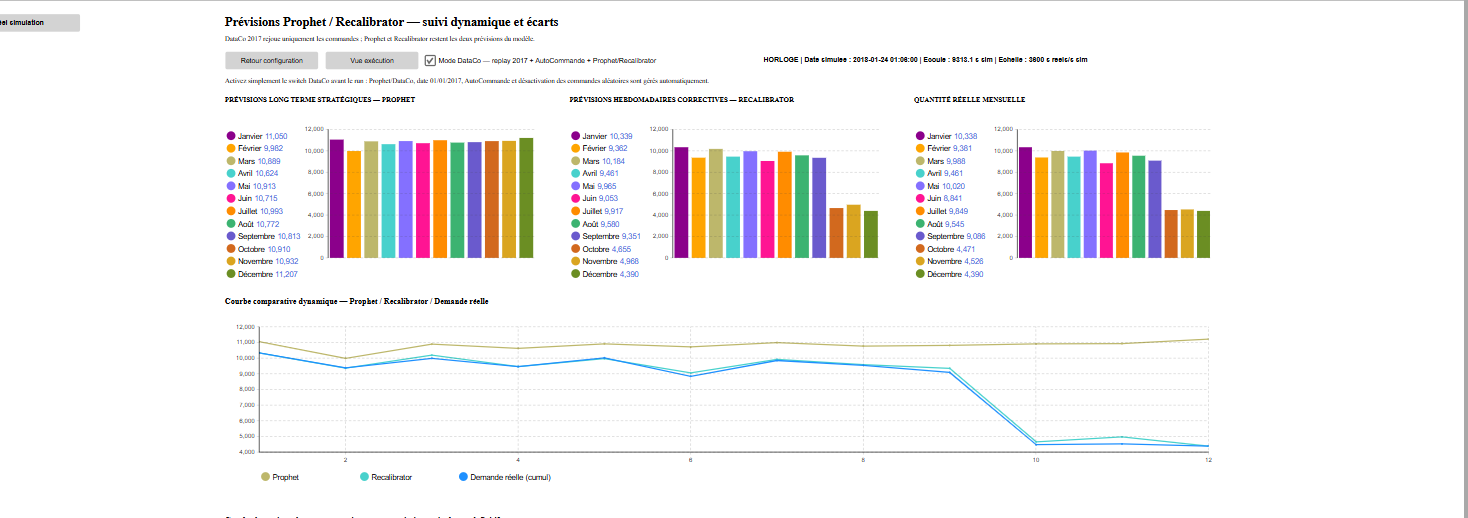
\includegraphics[width=\textwidth]{documentation/assets/dataco_final_run/screenshots/05_reference_dashboard_3600.png}
\caption{Tableau de bord Prophet / Recalibrator / demande réelle, campagne de référence RUN 1 (\code{simToRealSeconds = 3600}).}
\label{fig:dashboard}
\end{figure}

\subsection{Interprétation}

Le dernier trimestre illustre le rôle du Recalibrator. En octobre, Prophet maintient une anticipation d'environ 10\,910 unités alors que la demande réelle s'établit à 4\,471 unités : la prévision initiale reste proche du régime appris sur 2015--2016 et ne peut pas, par construction, anticiper un changement de régime survenant en cours d'année. Le Recalibrator ramène la prévision à environ 4\,655 unités, soit une erreur résiduelle d'environ 183,71 unités contre environ 6\,438,6 unités pour Prophet seul. Le mécanisme ne remplace pas Prophet ; il transfère progressivement le poids de la prévision vers la demande observée à mesure que celle-ci devient disponible, ce qui est précisément l'objet de la section suivante.

\section{Justification du facteur de confiance \texorpdfstring{$\alpha_j$}{alpha\_j}}

\subsection{Problème de recalibration}

Le Recalibrator combine deux informations à chaque cycle : la prévision Prophet de référence $F_P$, calculée avant l'exécution, et une projection $F_{proj}(j)$ construite à partir de la demande réellement observée depuis le début du mois. Au début du mois, peu de données sont observées et la projection réelle est fragile ; à mesure que $j$ augmente, davantage d'information est disponible et la confiance dans la projection croît. Le problème consiste à définir un poids $\alpha_j \in [0,1]$ qui gouverne cette transition.

\subsection{Projection run-rate}

Le rythme moyen observé jusqu'au jour $j$ s'écrit $r_j = R_j/j$, où $R_j$ est la demande cumulée observée au jour $j$. La projection de fin de mois prolonge ce rythme sur les $N-j$ jours restants :
\[
F_{proj}(j) = R_j + r_j\,(N-j) = R_j\times\frac{N}{j}
\]
Exemple : pour $R_j=4\,500$ au jour $j=10$ d'un mois de $N=30$ jours, $r_{10}=450$ unités par jour et $F_{proj}(10)=4\,500\times30/10=13\,500$ unités.

\subsection{Forme générale du facteur de pondération}

Le facteur de confiance appartient à la famille générale $\alpha_j=(j/N)^{\gamma}$, avec $\gamma>0$. Le Recalibrator retient $\gamma=1/2$ :
\[
\boxed{\alpha_j = \sqrt{\frac{j}{N}}}
\]
Ce choix est présenté comme un choix de conception motivé par les propriétés développées ci-dessous, et non comme un théorème établissant un optimum universel.

\subsection{Propriétés mathématiques}

\paragraph{A. Bornage.} Pour $0\le j\le N$, $0\le j/N\le1$, donc $0\le\alpha_j\le1$.

\paragraph{B. Extrémités.} $\alpha_0=0$ et $\alpha_N=1$ : en début de mois, Prophet porte la prévision ; en fin de mois, la projection issue du réel la porte entièrement.

\paragraph{C. Monotonie.}
\[
\frac{d\alpha}{dj} = \frac{\gamma}{N}\left(\frac{j}{N}\right)^{\gamma-1} > 0
\]

\paragraph{D. Concavité pour $\gamma=1/2$.}
\[
\frac{d^2\alpha}{dj^2} = \frac{\gamma(\gamma-1)}{N^2}\left(\frac{j}{N}\right)^{\gamma-2} < 0
\]

La confiance dans le réel augmente rapidement lorsqu'arrivent les premières observations, puis les gains marginaux diminuent à mesure que le mois avance.

\subsection{Pourquoi la racine carrée}

À mi-mois, $j/N=0{,}5$ : une progression linéaire donnerait $\alpha=0{,}5$, tandis que $\alpha_j=\sqrt{j/N}\approx0{,}707$. La racine carrée accorde donc plus rapidement du poids aux observations réelles qu'une montée linéaire.

\begin{center}
\small
\begin{tabular}{lrr}
\toprule
Avancement du mois & Linéaire & $\sqrt{j/N}$ \\
\midrule
10\,\% & 0,10 & 0,316 \\
25\,\% & 0,25 & 0,500 \\
50\,\% & 0,50 & 0,707 \\
75\,\% & 0,75 & 0,866 \\
100\,\% & 1,00 & 1,000 \\
\bottomrule
\end{tabular}
\end{center}

\subsection{Combinaison convexe}

La prévision recalibrée combine les deux estimateurs selon leur poids respectif :
\[
F_{recal}(j) = (1-\alpha_j)\,F_P + \alpha_j\,F_{proj}(j)
\]
Puisque $0\le\alpha_j\le1$, cette expression est une combinaison convexe des deux estimations : $F_{recal}(j)$ reste toujours compris entre $F_P$ et $F_{proj}(j)$, sans saut brutal de l'une à l'autre. $\alpha_j$ est un poids de confiance temporel, pas une probabilité \emph{a posteriori} : la formulation relève d'une combinaison pondérée adaptative, dans l'esprit des combinaisons de prévisions étudiées dans la littérature \cite{batesgranger1969,timmermann2006}, et non d'une inférence bayésienne conjuguée.

\subsection{Exemple numérique}

Avec $F_P=11\,000$, $F_{proj}=13\,500$ et $\alpha_{15}\approx0{,}707$ :
\begin{align*}
F_{recal} &= 0{,}293\times 11\,000 + 0{,}707\times 13\,500 = 12\,767{,}5 \text{ unités.}
\end{align*}
À mi-mois, les observations portent déjà 70,7\,\% du poids de la prévision recalibrée.

\subsection{Validation empirique et portée de la justification}

Les propriétés A à D justifient la cohérence de la forme choisie : bornage, transition progressive, confiance croissante et concave. Les résultats du RUN 1 montrent l'efficacité empirique du mécanisme complet : la MAE passe de 2\,491,89 à 123,06 unités, le MAPE de 45,75\,\% à 1,91\,\%, le RMSE de 3\,441,15 à 180,71. Ces résultats ne démontrent cependant pas que $\gamma=0{,}5$ est l'unique ou le meilleur réglage universel. Une analyse de sensibilité sur $\gamma\in\{0{,}3,\,0{,}5,\,0{,}7,\,1{,}0\}$ permettra de compléter la validation du choix et d'en étudier la robustesse.

\section{Méthodologie d'optimisation}

\subsection{Conditions nécessaires pour parler d'optimisation}

Pour parler d'optimisation, six éléments doivent être définis : des variables de décision, des objectifs, des contraintes, une politique de référence, une méthode de recherche, et une validation comparative et statistique.

\subsection{E4 -- optimisation ZENER}

E4 prend pour baseline le scénario perturbé E2. Les variables de décision couvrent la capacité du poste critique $x_1\in\{1,2,3\}$, la taille des sous-lots $x_2\in\{25,50,100,200\}$, la règle de priorité $x_3\in\{\text{FIFO, EDD, priorité ordinaire, hybride}\}$ et la politique de stock $x_4\in\{\text{actuel},+25\%,+50\%\}$, soit $3\times4\times4\times3=144$ configurations candidates. Cinq objectifs sont poursuivis simultanément : minimiser le nombre de commandes en retard, minimiser le WIP moyen, minimiser le délai de traitement (OFCT), minimiser le coût total, et maximiser le Performance Index. Les contraintes imposent un stock non négatif, une charge inférieure ou égale à la capacité installée, la satisfaction de la demande dans les limites définies par le modèle, un budget lorsqu'il est activé, un niveau de service minimal, et une condition terminale commune à toutes les configurations comparées.

\subsection{E5 -- optimisation DataCo fondée sur la prévision}

E5 est un protocole expérimental qui n'a pas encore été exécuté. Il compare quatre politiques de pilotage :

\begin{center}
\small
\begin{tabularx}{0.92\textwidth}{lX}
\toprule
Politique & Description \\
\midrule
P0 & Réactive, sans prévision (référence) \\
P1 & Pilotée par Prophet seul \\
P2 & Pilotée par Prophet et Recalibrator \\
P3 & Pilotée par Prophet, Recalibrator et paramètres de planification et de stock optimisés selon le protocole E5 \\
\bottomrule
\end{tabularx}
\end{center}

Pour chaque famille simulée $p$, le vecteur de décision est $x_p=(SS_p,\,s_p,\,Q_p,\,f_p)$, où $SS_p$ est le stock de sécurité, $s_p$ le point de commande, $Q_p$ la quantité de réapprovisionnement et $f_p$ la fréquence de révision du plan. $Q_p$ n'est pas qualifié de quantité économique : dans le protocole E5, c'est une variable de décision à optimiser, pas une couverture fixe.

\subsection{Fonction objective et contraintes}

\[
\min\; C_{\text{total}} = \sum_{p,t} \Big[ h_p\, I_{p,t} + b_p\, B_{p,t} + K_p\, y_{p,t} + c_p\, Q_{p,t} \Big]
\]
où $I_{p,t}$ est le niveau de stock de la famille $p$ en fin de période $t$, $B_{p,t}$ la rupture ou le retard cumulé, $y_{p,t}$ une variable indicatrice de déclenchement d'un ordre de réapprovisionnement, et $h_p$, $b_p$, $K_p$, $c_p$ respectivement le coût de possession, le coût de rupture, le coût fixe de commande et le coût unitaire de la famille $p$. Les contraintes sont un niveau de service minimal par famille $\text{NiveauDeService}_p \geq SL_p^{\min}$, une capacité de réapprovisionnement bornée $Q_{p,t} \leq \text{Capacite}_{p,t}$, et une équation de bilan de stock $I_{p,t} = I_{p,t-1} + Q_{p,t} - D_{p,t}$, où $D_{p,t}$ provient de la chaîne de prévision et de recalibration décrite section~1.

\subsection{Recherche des solutions et Pareto}

Pour E4, l'exploration factorielle des 144 configurations identifie les solutions Pareto-efficaces : une solution est dominée lorsqu'une autre lui est au moins équivalente sur tous les objectifs et strictement meilleure sur au moins un.
\begin{center}
\small
144 configurations $\to$ simulation $\to$ calcul des KPI $\to$ filtre des contraintes $\to$ solutions admissibles $\to$ front de Pareto.
\end{center}

\subsection{Sélection AHP}

L'AHP intervient après la construction du front de Pareto, pour sélectionner parmi les solutions Pareto-efficaces le compromis correspondant aux priorités décisionnelles retenues par les experts. L'AHP ne recherche pas les configurations ; il sélectionne un compromis managérial parmi des solutions déjà Pareto-efficaces, en aval de la recherche d'optimisation proprement dite.

\subsection{Validation statistique}

Pour toute configuration retenue en E4 ou E5, la validation prévoit plusieurs réplications par configuration, avec des graines aléatoires communes entre configurations comparées, un arrêt lorsque la demi-largeur de l'intervalle de confiance à 95\,\% du critère principal descend sous un seuil fixé a priori (par exemple 5\,\% de la valeur moyenne estimée), puis une validation croisée sur de nouvelles graines indépendantes de celles utilisées pour la sélection. Pour chaque comparaison sont rapportés la moyenne, l'écart-type, l'intervalle de confiance à 95\,\%, la différence absolue et relative, un test statistique apparié adapté au plan d'expérience, une taille d'effet, et une vérification de robustesse sur plusieurs intensités de perturbation. Pour E4, la robustesse est étudiée notamment sur une demande exceptionnelle $\in\{100,150,200,250\}$, et pourra être étendue à un retard fournisseur, une panne machine, une variabilité du temps de traitement et une demande ordinaire accrue.

\subsection{Condition terminale}
\label{sec:condition-terminale}

365 commandes générées ne signifient pas expérience terminée. Sur le RUN 1, 365 commandes ont été générées, 79 sont closes et 286 restent EN\_ATTENTE. Les métriques Prophet et Recalibrator sont d'ores et déjà évaluables, car les douze mois de demande sont disponibles ; en revanche, le Performance Index, le taux de service, les délais, les coûts et les quantités livrées ne sont pas encore des résultats terminaux. Pour E5, la campagne devra attendre que toutes les commandes soient closes, que tous les réapprovisionnements soient terminés, et qu'aucun encours pertinent ne subsiste avant de mesurer la performance des politiques comparées.

\subsection{Prérequis graine aléatoire}

Le manifeste runtime actuel indique \code{graineAleatoire = NON\_ACCESSIBLE\_DANS\_MAIN} : les nombres aléatoires communs ne sont pas encore opérationnels sur les runs déjà exécutés. Pour E4 et E5, le protocole prévoit d'exposer et de contrôler explicitement la graine de l'expérience AnyLogic avant la campagne d'optimisation, de sorte que $\text{Seed}_{k,P_0} = \text{Seed}_{k,P_i}$ pour les politiques comparées lors d'une même réplication $k$. Cette exposition est un prérequis technique du protocole futur, pas un résultat déjà obtenu.

\subsection{Portée scientifique des conclusions}

La formulation retenue pour toute configuration issue de ce protocole est « meilleure configuration identifiée dans l'espace de décisions exploré », et non « optimum global », sauf preuve mathématique ou exploration exhaustive d'un espace complet qui permettrait réellement cette conclusion. E5 n'a pas encore été exécutée : le protocole prévoit la comparaison des politiques P0 à P3, et la campagne devra en mesurer les résultats après extinction complète des flux résiduels.

\section{Synthèse}

Prophet fournit une prévision mensuelle de référence entraînée sur 2015--2016 et appliquée à 2017 ; DataCo exécute la demande sous forme de commandes clientes journalières qui traversent le pipeline Source, Make, Deliver ; le Recalibrator combine cette prévision à la demande observée au moyen d'un facteur $\alpha_j=\sqrt{j/N}$ dont les propriétés de bornage, de monotonie et de concavité justifient la forme, et dont l'efficacité empirique est mesurée sur le RUN 1 par une réduction de l'erreur absolue totale d'environ 95,06\,\%. La démarche d'optimisation de SCONTO-SVU s'appuie sur E4, déjà mené selon un protocole complet d'exploration factorielle, de front de Pareto et de sélection AHP, et sur E5, un protocole formalisé pour la planification multi-produit fondée sur la prévision, dont l'exécution et la validation statistique restent à mener une fois la condition terminale atteinte et la graine aléatoire exposée.

\begin{thebibliography}{9}
\small
\bibitem{taylor2018forecasting} Taylor, S. J., \& Letham, B. (2018). Forecasting at Scale. \emph{The American Statistician}, 72(1), 37--45. DOI: 10.1080/00031305.2017.1380080.
\bibitem{batesgranger1969} Bates, J. M., \& Granger, C. W. J. (1969). The Combination of Forecasts. \emph{Operational Research Quarterly}, 20(4), 451--468.
\bibitem{timmermann2006} Timmermann, A. (2006). Forecast Combinations. In \emph{Handbook of Economic Forecasting}, Vol. 1, 135--196. Elsevier.
\bibitem{hadleywhitin1963} Hadley, G., \& Whitin, T. M. (1963). \emph{Analysis of Inventory Systems}. Prentice-Hall, Englewood Cliffs, N.J.
\end{thebibliography}

\end{document}
